\section{Scaling at Risk: Challenges of Data and Computing Power}
\subsection{The Ceiling of Public Data}
\label{subsec:data_exhaustion}
\paragraph{Public data for pretraining is exhausting.} The rapid advancement of large language models has created an insatiable appetite for training data. Scaling laws establish that model performance improves predictably with data quantity—a relationship that demands exponentially growing datasets \cite{hoffmann2022training}. A canonical example is GPT-3, trained on {300 billion tokens} spanning books, web content, and programming code \cite{brown2020language}. Current projections suggest dataset sizes grow at 0.38 orders of magnitude (2.4$\times$) annually \cite{villalobos2022trends}, implying models will require {three orders of magnitude more data} within a decade. \looseness-1

Despite the internet's vast textual resources, the total stock of high-quality human-generated text remains bounded. Recent estimates place this limit at approximately {$4\times 10^{14}$ tokens} \cite{villalobos2022trends}. \cite{villalobos2024will} argues that current consumption patterns suggest exhaustion of public text data by 2028, potentially accelerated to 2026 through excessive data reuse during training (a practice termed {overtraining}). 
% This creates a fundamental tension: while additional data currently drives progress, unrestrained consumption threatens future advancement.
Therefore, the finite nature of publicly available human-generated text data is expected to become a major bottleneck for LLM scaling within the next decade. Despite the current large scale of public data, the risk of data exhaustion is rapidly approaching as data demand continues to grow \cite{sevilla2022compute}.

% Synthetic data generation presents a paradoxical opportunity. 
\paragraph{Synthetic data has potential but faces challenges.}
Faced with the threat of data exhaustion, researchers have proposed various solutions, among which synthetic data generation is considered one of the most promising approaches. 
By leveraging LLMs to produce their own training data, researchers envision {self-sustaining data ecosystems}. Early successes in constrained domains like mathematics and code generation, where automated verification ensures quality, demonstrate potential \cite{liu2023tinygsm}.  Recent work \cite{chen2024diversity} demonstrated that diverse synthetic data enhances the performance of LLMs during both pre-training and fine-tuning.


The adoption of synthetic data faces three fundamental challenges. First, \textit{model collapse} occurs when models iteratively train on their own outputs, causing gradual divergence from original data distributions. This recursive process amplifies biases and reduces output diversity, ultimately degrading model performance across generations \cite{shumailov2023curse,dohmatob2024strong}. 
Second, \textit{synthetic data quality} remains inherently unverifiable in open-domain contexts. While formal domains like mathematics allow algorithmic validation, natural language lacks objective evaluation standards. The absence of ground-truth verification creates self-referential quality assessments, compromising reliability \cite{alemohammad2023self,wenger2024ai}.
Finally, synthetic data struggles to replicate human \textit{linguistic diversity}. Current methods disproportionately replicate dominant language patterns while underrepresenting cultural nuances and low-frequency expressions. This homogeneity limits their utility for training robust general-purpose models \cite{fan2024scaling}.

These persistent challenges underscore that synthetic data alone cannot sustainably address the looming data scarcity crisis, compelling the research community to seek complementary strategies that transcend conventional data acquisition paradigms.




\subsection{The Monopoly of Computing Resources}\label{subsec:compute_monopoly}
\paragraph{A few AI giants dominate the computing power.}
The AI computing landscape is dominated by a few major tech giants like OpenAI, Google, Microsoft, and Meta, which control powerful hardware such as GPUs and TPUs. This monopolization creates a significant barrier for smaller AI startups and research institutions, who struggle to access such advanced resources. Additionally, these companies control proprietary AI models, datasets, and software frameworks that require immense computing power, further widening the gap between the giants and smaller players. As a result, high-performance computing resources remain increasingly inaccessible to anyone outside these dominant entities.

\begin{wrapfigure}{r}{0.5\linewidth}
    \vspace{-12pt} % Adjust vertical space if needed
    \centering
    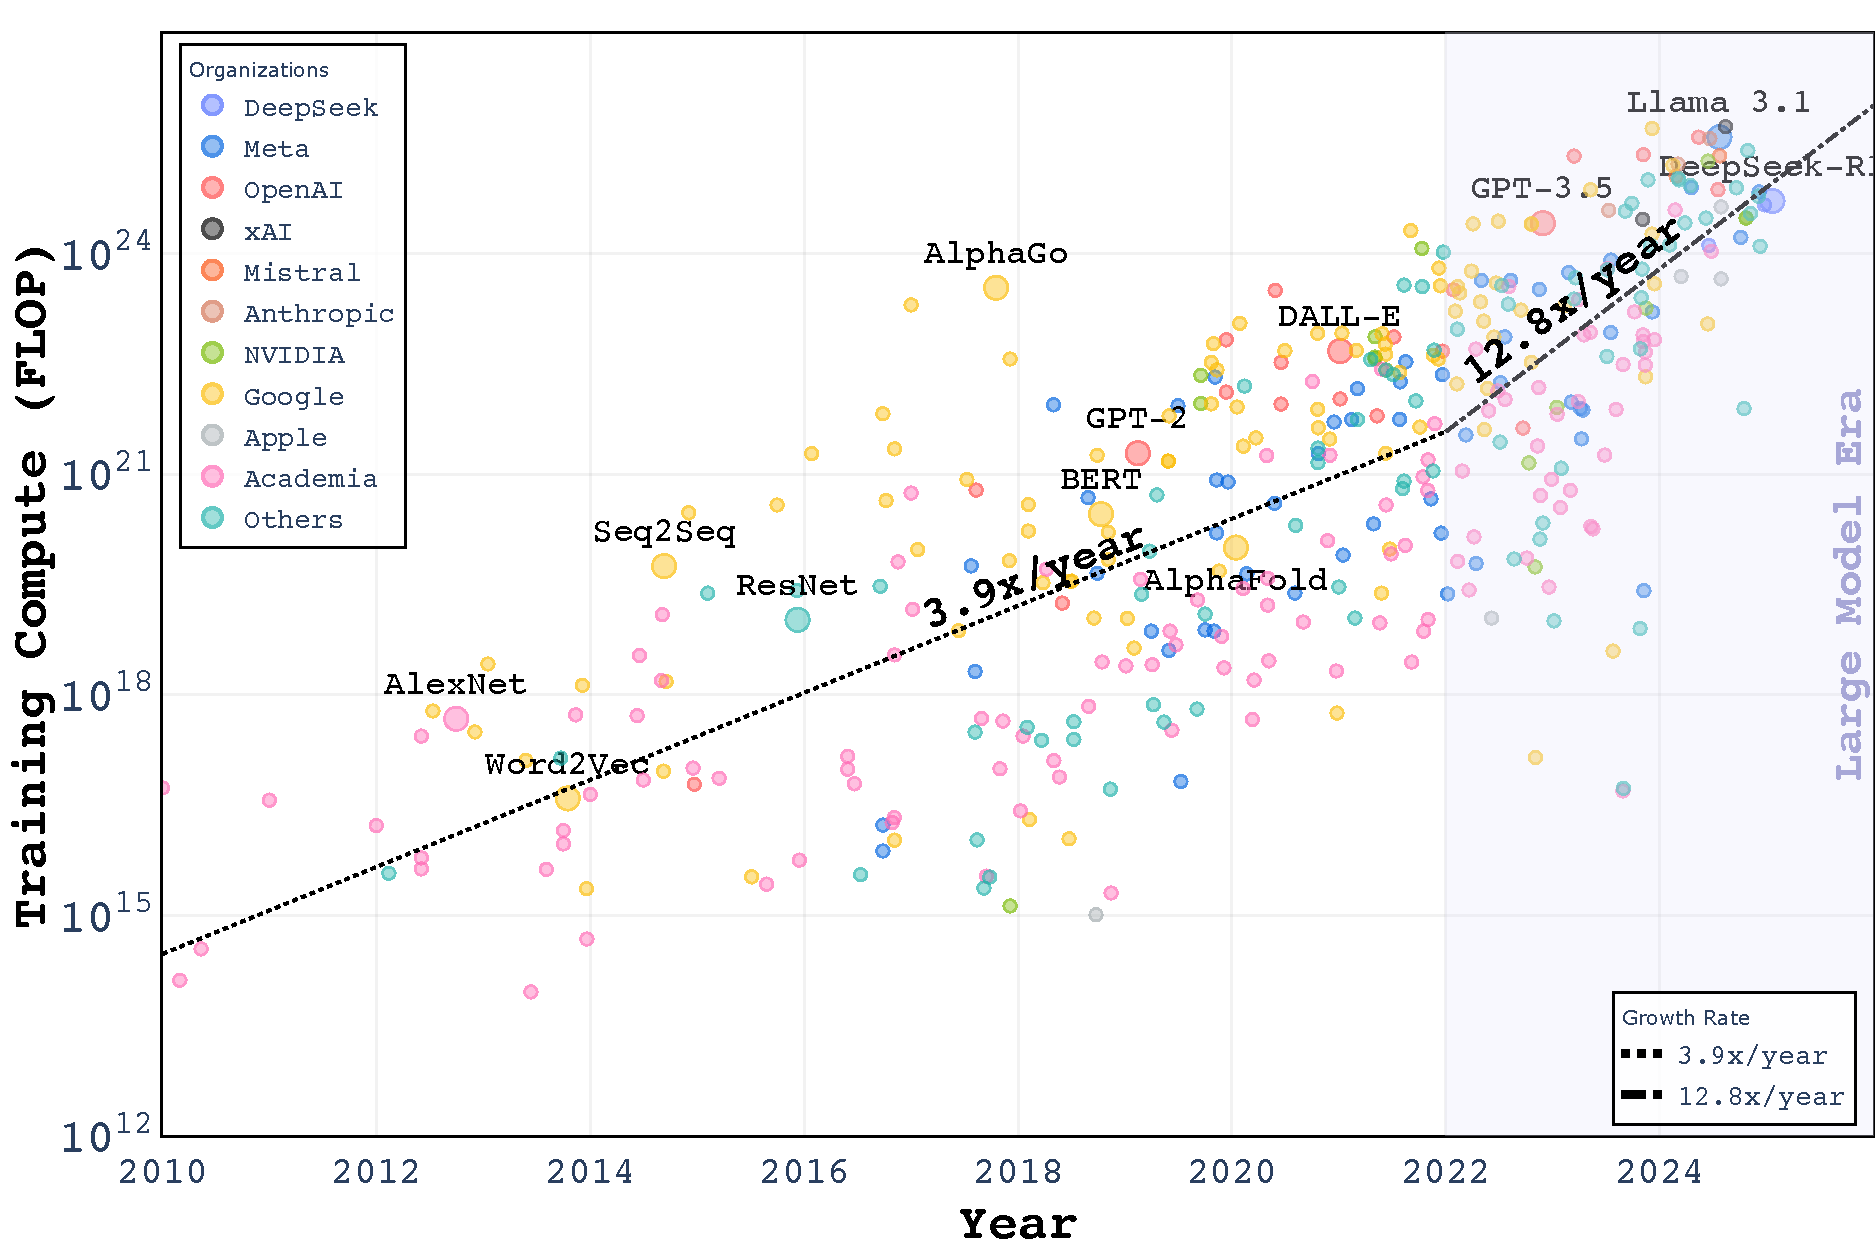
\includegraphics[width=\linewidth]{figs/ai_compute_trend.pdf}
    \vspace{-15pt} % Adjust vertical space if needed
    \caption{Trend of Computational Demand for Model Training. (Data source:~\cite{epoch2023trendsinmachinelearninghardware}).}
    \label{fig:model_comput_trend}
    \vspace{-12pt} % Adjust vertical space if needed
\end{wrapfigure}

\paragraph{Computational demand is growing exponentially.}
As large-scale AI models like GPT-4~\cite{openai2023gpt4}, Llama 3~\cite{meta2024llama3.1}, and DeepSeek-V3~\cite{liu2024deepseek} surpass the trillion-parameter scale, the global AI landscape faces severe computational efficiency challenges. As shown in Figure~\ref{fig:model_comput_trend}, since the deep learning revolution in 2010, AI training demands have grown at a super-exponential rate of 3.9$\times$ per year—an acceleration that intensified with the adoption of the transformer architecture as the industry standard \cite{vaswani2017attention}. With the advent of the era of large language models in 2022, the demand for computing power has surged even further, reaching an unprecedented growth rate of 12.8$\times$ per year. This marks a transformative shift in AI computation, where the need for computing power is expanding at an unprecedented pace, pushing the limits of existing hardware and infrastructure. \looseness-1




\paragraph{Moore's Law is slowing down.}
Moore's Law, which has driven the growth in computing power for decades, is slowing down as we approach the physical limits of silicon-based chip technology~\cite{kressel2023end}. The difficulty in shrinking transistors has led to diminishing returns in computational performance. As a result, the AI industry is relying more on specialized hardware like GPUs, TPUs, and custom chips to meet growing demands. However, this shift has made high-performance hardware even more expensive and exclusive, further intensifying the gap between organizations with the resources to develop advanced AI models and those without.

\paragraph{Infrastructure capacity is a constraint.}
The rapid expansion of AI model scales and the surge in computational demand are facing dual constraints in global computing infrastructure. On one hand, bottlenecks in advanced semiconductor manufacturing severely limit the expansion rate of AI data centers. The foundry capacity for wafers at 5nm and below—such as those produced by TSMC—has already been fully booked by leading technology companies until 2026~\cite{benzinga2024tsmc}. Moreover, the construction of new wafer fabs involves long lead times and is further constrained by the global supply chain shortages of critical equipment, such as lithography machines.
On the other hand, the exponential increase in chip deployment within individual AI clusters is putting immense pressure on the already limited semiconductor manufacturing capacity, pushing the industry toward its production ceiling~\cite{scaleflux2024ai}.
These factors have significantly hindered the continuous expansion of computing power, making it increasingly difficult to scale AI infrastructure sustainably.
